\documentclass[11pt, oneside]{article}
\usepackage[margin=1in]{geometry}
\geometry{letterpaper}
\usepackage{booktabs}
\usepackage{hyperref}
\usepackage{enumitem}
\usepackage{float}
\usepackage{caption}
\usepackage{subcaption}
\usepackage[numbers]{natbib}
\usepackage{graphicx}
\usepackage{amssymb}
\usepackage{amsmath}
\usepackage{array}
\usepackage{longtable}
\usepackage{xcolor}
\usepackage{tabularx}
\usepackage{setspace}
\usepackage{microtype}
\emergencystretch=2em
\newcolumntype{Y}{>{\raggedright\arraybackslash}X}
\captionsetup{font=small}
\hypersetup{colorlinks=true,linkcolor=blue,citecolor=blue,urlcolor=blue}
\newcommand{\NR}{\textit{NR}}
\title{CS781 Capstone Project:\\ In-House Legal Intelligence System}
\author{Anirudh Bankhede\\240131\\{\tt anirudhb24@iitk.ac.in}\\Indian Institute of Technology Kanpur (IIT Kanpur)}
\date{}
\begin{document}
\maketitle
\begin{abstract}
This project explores how far a small, self-hosted legal NLP system can go under limited GPU compute. It covers seven tasks, from text continuation and entity extraction to summarization and prior-case retrieval. Four foundation models, with 52.2--82.0 million parameters, were trained from scratch on the official legal corpus and then adapted to the downstream tasks. The experiments compare full and partial tuning with low-rank methods, adapters, prompts and distillation. The main findings concern exact span boundaries, long-document coverage and the reliability of validation scores. Summarization reached an audit BERTScore F1 of 0.82624, while retrieval reached tuning micro F1@7 of 0.34367. Several more complex methods failed to improve on simpler alternatives. The report separates local measurements from official competition results and documents how training was resumed after interruptions.
\end{abstract}

\section{Competition Result}
\noindent\textbf{Codabench username:} a\_240131\hfill\textbf{Roll number:} 240131

\begin{table}[H]
\centering\small
\caption{Official Codabench scores, ranks and valid submission counts on 9 November 2026.}
\label{tab:leaderboard}
\begin{tabular}{clccc}
\toprule
Phase & Task & Primary score & Rank & Valid submissions\\
\midrule
1 & Legal LM pretraining & 0.8257 & 115 & 4\\
2 & Legal NER & 0.5276 & 65 & 6\\
3 & Rhetorical roles & 0.5058 & 59 & 6\\
4 & Judgment prediction & 0.7553 & 43 & 6\\
5 & Statute identification & 0.3777 & 62 & 6\\
6 & Summarization & 0.8234 & 116 & 6\\
7 & Prior-case retrieval & 0.3077 & 101 & 7\\
\bottomrule
\end{tabular}
\end{table}

\noindent\textbf{Total valid Codabench submissions across all phases:} 41.\quad\textbf{Date recorded:} 9 November 2026.
\medskip
The competition required at least four distinct submissions in each phase. The recorded counts meet that minimum: four in Phase~1, six each in Phases~2--6 and seven in Phase~7, for a total of 41 valid submissions.

The public code repository is
\href{https://github.com/anirudh3810/cs781-capstone-legal-intelligence}{\texttt{anirudh3810/cs781-capstone-legal-intelligence}}.
The repository contains the notebooks, source code, saved numerical evidence and instructions needed to run each phase. Section~\ref{sec:results} explains the local results and how they relate to the official scores.

\section{Introduction and Problem Description}
The aim of this project was to build a legal NLP system that could run with compact models and limited compute. Legal documents made this difficult in several ways: they are long, repeat procedural details and often place decisive information among citations and arguments. A self-hosted setup also makes the origin of the data and model weights easier to track.

The seven phases address different parts of this problem. Phase~1 generates a 128-word continuation from a legal prompt and uses BERTScore F1. Phase~2 extracts exact character spans for twelve entity types, scored by strict macro F1. Phase~3 labels each supplied sentence with its rhetorical role. Phases~4 and~5 predict a binary judgment outcome and a set of statute IDs respectively; both use macro F1. Phase~6 generates summaries, evaluated with BERTScore and ROUGE. Phase~7 retrieves exactly seven prior cases per query and uses micro F1@7.

The foundation models had to stay within 50M--300M parameters and be trained from scratch on the official data. These constraints shaped the experiments: how much context to retain, where to adapt the backbone, and when further training was worth its cost. Each downstream task starts from Phase~1 independently. Building a deployed application or feeding predictions from one phase into the next was outside the scope of the project.

\section{Data Analysis and Preprocessing}
\subsection{Sources and official splits}
All training text comes from the official course release~\cite{course}. The foundation corpus contains Acts, High Court, Supreme Court and Tribunal documents; later phases use their own task-specific files. Test labels were excluded from fitting and model selection. Table~\ref{tab:data} lists the loaded splits. For NER, the two public labeled files were combined for document-fold experiments. For summarization, two of 7,030 rows had no reference summary and were skipped, leaving 7,028 labeled cases.

\begin{table}[H]
\centering\small
\caption{Task data recovered from saved audits. A dash denotes an unlabeled or inapplicable split. The Phase~7 candidate pools are split-specific.}
\label{tab:data}
\begin{tabular}{clrrr}
\toprule
Phase & Unit & Train & Dev & Test\\
\midrule
2 & Documents & 35 & 35 & 35\\
3 & Documents / sentences & 80 / 16,845 & 10 / 2,142 & 10 / 2,197\\
4 & Case rows & 37,387 & 3,505 & 1,517\\
5 & Case rows & 42,750 & 10,181 & 13,019\\
6 & Labeled cases & 7,028 & -- & 100\\
7 & Queries & 827 & 118 & 237\\
7 & Candidate cases & 4,320 & 1,023 & 1,727\\
\bottomrule
\end{tabular}
\end{table}

\subsection{Corpus statistics that actually informed design}
Bases~02 and~04 use 39,921 deduplicated documents: 9,981 Acts, 9,952 High Court, 9,991 Supreme Court and 9,997 Tribunal documents. Their word totals are very different: 62.19M, 5.66M, 37.65M and 11.28M respectively. Equal document sampling therefore does not give equal token exposure. Base~03 uses 31,946 documents, while base~01's larger corpus audit contains 3,356,594. The tokenizer audit covers only the first 256 training documents, all Acts, so it cannot describe token usage across the whole corpus.

The label counts also affect how the scores should be read. Phase~3 has only three \emph{PrecedentOverruled} sentences, all from one document, and 284 \emph{Dissent} sentences from two documents. In Phase~4, the 37,387 training rows include 22,067 negative and 15,320 positive outcomes, 5,735 exact duplicate rows and 31,652 case groups. The median document is 13,023 characters long; the 95th percentile is 54,753. Phase~5 has 100 labels, with training support ranging from 272 to 11,730 positives. A case has three labels at the median and eight at the 95th percentile. These differences make grouped validation and per-label calibration important.

\begin{figure}[H]
\centering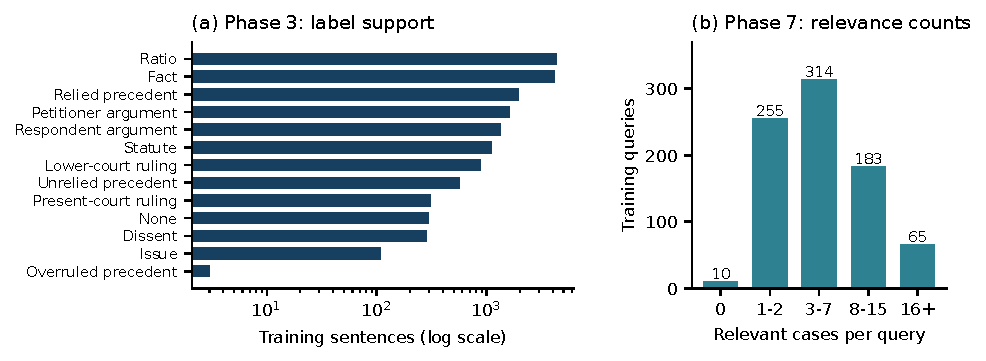
\includegraphics[width=\textwidth]{figures/data_distributions.pdf}
\caption{Aggregate distributions computed from the saved training audits. Rare rhetorical roles concentrate in very few independent documents. Retrieval relevance cardinality spans both sides of the required seven predictions.}
\label{fig:data}
\end{figure}

Long inputs are especially important in the last two tasks. Summarization sources have a median length of 17,911 characters, while references have a median of 638 words and a 95th percentile of 2,010. Retrieval queries have median lengths of 4,508, 4,619.5 and 4,653 words in train, dev and test. They average 6.42 and 8.25 relevant cases in train and dev. Candidate lengths exceed 19,000 words at the 95th percentile in every split. Court and date patterns were not analyzed well enough to justify adding temporal features.

\subsection{Preprocessing}
For NER, the original Unicode text is kept intact so that normalization cannot silently shift character offsets. BPE positions are mapped back to the original character boundaries; 8,241 of 8,393 gold spans match exactly after trimming whitespace. Phase~3 uses the supplied sentence boundaries. Longer cases are split into overlapping chunks, while summarization first selects sentences to fit its source budget. Retrieval uses the same chunk policy for queries and candidates and keeps IDs as strings, preserving leading zeros. Duplicate texts are grouped together during validation.

\section{Approach and Model Evolution}
\subsection{Phase-1 foundation model}
The four foundation models test different attention patterns within the parameter budget~\cite{vaswani2017attention}. Their dimensions are listed in Table~\ref{tab:foundations}, and parameter counts were checked at runtime. Bases~03 and~04 use RoPE and RMSNorm~\cite{su2021roformer,zhang2019rmsnorm}; base~04 also shares key/value heads~\cite{ainslie2023gqa}. Byte-level BPE avoids a fixed word vocabulary for names and legal citations. Bases~01/02 use 32k tokenizers, and bases~03/04 use separate 25k tokenizers.

\begin{table}[H]
\centering\small
\caption{Foundation architectures and completed training counters. FFN is the intermediate feed-forward width; contexts are architecture limits. Processed tokens count repeated training exposure, not unique corpus tokens.}
\label{tab:foundations}
\begin{tabular}{clrrrrr}
\toprule
Base & Family & Layers & Width / heads & FFN & Context & Params (M)\\
\midrule
01 & Causal & 8 & 768 / 12 & 2048 & 1024 & 82.012\\
02 & Encoder--decoder & 6+6 & 512 / 8 & 2048 & 1024/512 & 61.343\\
03 & Prefix hybrid & 24 & 384 / 6 & 1024 & 1280 & 52.206\\
04 & Local/global causal & 14 & 512 / 8Q:2KV & 1536 & 1536 & 55.113\\
\bottomrule
\end{tabular}
\end{table}

All four models minimize target cross-entropy, with held-out documents, tied embeddings and equal-probability source draws. Bases~01--04 completed 12k, 12k, 10k and 15k steps, processing 74.41M, 242.87M, 203.01M and 304.58M tokens. Base~04 combines a 256-token local window with a global anchor every 128 positions. Submission generation uses greedy cached decoding with a 128-word target. Since the runs differ in corpus subset, tokenizer and objective, their losses are not a controlled comparison of architecture alone.

\begin{figure}[H]
\centering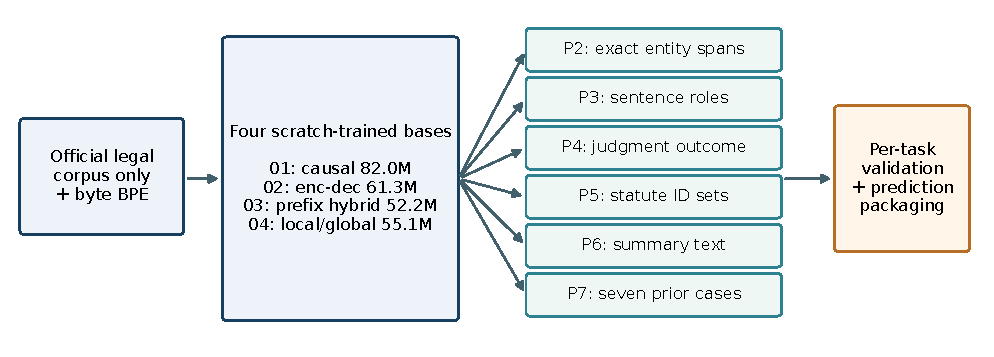
\includegraphics[width=\textwidth]{figures/architecture.pdf}
\caption{Actual transfer structure. Each downstream phase starts from an original foundation and trains its own head or adaptation. The tasks are separate descendants, rather than a seven-stage inference cascade.}
\end{figure}

\subsection{Transfer protocol (Phases 2--7)}
The downstream experiments vary how much of the foundation model is updated. Full tuning changes the backbone, while partial tuning changes only upper blocks. LoRA adds a low-rank update~\cite{hu2021lora}; LoRMA instead applies an identity-initialized multiplicative transformation to a frozen matrix~\cite{bihany2025lorma}. Other variants use bottleneck adapters~\cite{houlsby2019adapters}, activation scales~\cite{liu2022ia3} or soft prompts~\cite{lester2021prompt}. The adaptive-rank modules use an importance-based masking schedule inspired by AdaLoRA~\cite{zhang2023adalora}, rather than an exact reproduction of it. Distillation uses a teacher trained only on fitting data~\cite{hinton2015distill}. The README records the base and method for every slot.

\subsection{Phase 2 - Legal NER}
The first six NER methods use BIOUL tagging followed by character-boundary refinement. Later versions score span starts, ends and pairs directly in 384-token windows, with stride 288 and a 64-token span limit. V2 adds residual refinement and upper-layer tuning. V3 starts from V2, adds multiplicative start/end interactions and a residual pair network, and unfreezes twelve upper blocks. The final decoder selects a candidate source for each label from the raw and reranked V2/V3 outputs, then resolves overlaps and restores character offsets. Three document folds guide checkpoint and threshold selection. The reason for moving toward span extraction was practical: no threshold can recover a correct span that the candidate generator never proposes.

\subsection{Phase 3 - Rhetorical role prediction}
The initial role-prediction runs compare LoRA, rank-stabilized LoRA, IA$^3$, LoRMA, prompts and distillation. A later experiment fully tunes bases~03/01 with three-layer bidirectional GRU document heads, then selects a blend with earlier models on dev data. The separate HighF1 branch uses target-focused 448-token inputs, attention/mean/max pooling, position and domain embeddings, and a two-layer bidirectional GRU over twelve-sentence windows. Pair heads distinguish argument parties, precedent reliance and the source of a court ruling; a CRF adds transition scores. Five document folds favored raw decoding. Corporate Law and IT share the model, with a domain feature to distinguish them.

\subsection{Phase 4 - Court judgment prediction}
For judgment prediction, each case is represented by up to eight 640-token chunks. Features are projected to width 256, combined with position embeddings and passed through a one-layer chunk Transformer. Attention, mean and max pooling feed a binary classifier, with its threshold selected by macro F1. The six variants use full base~01, partial base~03, LoRMA base~04, adaptive-rank base~02, adapters base~03 and distilled base~03. Partial base~03 gives the best saved dev result at epoch~3 and threshold~0.55. The intended grouped outer folds did not finish, so this is a dev-selected result.

\subsection{Phase 5 - Legal statute identification}
Statute prediction combines pooled document features with the strongest chunk evidence for each label. Training uses four 512-token chunks; inference allows twelve, selected for coverage and statute cues. Sigmoids and calibrated thresholds return a label set. The six variants are partial base~03, full base~01, LoRMA base~04, adapters base~02, adaptive-rank base~03 and distilled base~03. Repeated gold statute IDs are deduplicated. All six reports are complete: slot~01 leads holdout macro F1 at 0.37934, with micro F1 0.48132 and subset accuracy 0.04143. Distillation in slot~06 is close at 0.37650 macro F1 and 0.47888 micro F1, with higher subset accuracy, 0.04515, and 32.0\% fewer trainable parameters, 15.08M versus 22.18M.

\subsection{Phase 6 - Abstractive summarization}
The summarization runs use LoRA, adaptive rank, LoRMA, Houlsby adapters, Pfeiffer adapters and sequence distillation on the original foundations. Source selection keeps section and legal-cue evidence within each model's context limit. References are capped at 480 tokens. Decoder-only models generate after the packed source; base~02 uses cross-attention. Greedy cached decoding includes length hints, a minimum output budget and repeated-ngram suppression. There is no separate candidate reranker. For distillation, a deterministic subset of fitting targets is replaced with summaries from the project teacher. BERTScore~\cite{zhang2020bertscore} is used only for evaluation.

\subsection{Phase 7 - Prior Case Retrieval (PCR)}
Retrieval uses a shared encoder to turn up to six 384-token chunks into normalized 256-dimensional vectors. The neural score gives equal weight to document cosine and the average best candidate-chunk match for each query chunk. Reciprocal rank fusion combines this ranking with full-document and passage BM25~\cite{cormack2009rrf}. The six variants use full base~03, partial base~01, LoRMA base~04, IA$^3$ base~02, prompted base~03 and distilled base~02. Known positives are excluded from negatives; one mining refresh and a fitting-only teacher provide additional supervision. Every output contains seven unique IDs. The proposed cross-encoder branch was not implemented.

\section{Experiments and Implementation Details}
\subsection{Compute and training protocol}
The runs were carried out on Kaggle using AdamW, mixed precision, gradient clipping, warmup and a decaying learning rate. Earlier experiments use two-GPU data parallelism; later classification and summarization use distributed jobs. Retrieval runs two independent experiments, one on each physical GPU. Inside a worker, \texttt{cuda:0} means its own visible device.

\begin{table}[H]
\centering\small
\caption{Settings of the selected local implementations. Epoch numbers denote selected checkpoints, not necessarily total executed passes. Batch settings are microbatch $\times$ accumulation; GPU world size is additional where applicable.}
\label{tab:hparams}
\begin{tabularx}{\textwidth}{clYYY}
\toprule
Phase & Selected variant & Input budget & Learning rate / batch & Selected training\\
\midrule
1 & B04 & 512 source +256 target & $2.5\!\times\!10^{-4}$; global 8$\times$4 & 15,000 steps\\
2 & V3 hybrid / B03 & 384/window, stride 288 & New pair $1.2\!\times\!10^{-4}$; batch 16 & Folds 24/18/24\\
3 & One-submission blend & 384/sentence in new branches & Backbone $1.3$--$1.5\!\times\!10^{-5}$; accum 4 & Dev-selected blend\\
4 & Partial / B03 & $8\times640$ chunks & $1.4\!\times\!10^{-5}$; case 1$\times$4 & Epoch 3\\
5 & Partial / B03 & $4\times512$ fit;12 infer & $1.4\!\times\!10^{-5}$; case 2$\times$2 & Epoch 7\\
6 & Adaptive rank / B03 & 760 source + controls; 480 target & $1.4\!\times\!10^{-4}$; probed batch$\times$4 & Epoch 3\\
7 & Full / B03 & $6\times384$ chunks & Backbone $2\!\times\!10^{-5}$, head $2\!\times\!10^{-4}$ & Epoch 2\\
\bottomrule
\end{tabularx}
\end{table}

Base~04 pretraining uses dropout 0.05, weight decay 0.1 and 500 warmup steps. Task heads generally use dropout 0.1--0.25 and weight decay 0.01; the exact values are in the code. NER V3 uses float32 with activation checkpointing. Later jobs use fp16 with a scaler on T4-class GPUs, or bf16 where supported. Retrieval probes long batches before training and reduces the batch after an OOM, preserving both the effective batch size and the saved position.

Recovering progress was important because a full suite could outlast one session. Checkpoints store trainable weights, optimizer, scaler, RNG and progress. Retrieval saves about every five minutes and after 18-minute segments; summarization saves about every ten minutes and after segments. The parent waits for workers to exit before replacing the recovery ZIP. Partial vectors, predictions and teacher outputs can also resume. The 8.5-hour retrieval guard stopped the supplied run during slot~05's fifth pass without marking it complete. Base~04 pretraining took 6.62 hours and the V3 span run 2.14 hours in their saved records; these timings do not apply to every configuration.

\subsection{Local evaluation}
The evaluation split matters as much as the displayed score. NER uses document folds, and role prediction reports both fixed thirteen-label and reference-supported macro F1. Judgment validation groups related cases and texts, although its outer folds are missing. Statute fitting/inner/holdout splits contain 31,994/4,311/6,445 rows. Summarization uses 6,324/352/352 fit/tune/audit cases. Retrieval divides dev into 83 tuning and 35 audit queries, but the supplied archive has no completed final audit.

\subsection{Ablations and controlled comparisons}
Some comparisons isolate a single change. Role-prediction decoders use the same logits, while the retrieval gold-only and KD students share initialization, schedule and matched steps for two passes. Comparisons across architectures also change capacity and adaptation, so they cannot explain the effect of one factor alone. There is no scratch-versus-transfer control that establishes a measured transfer gain.

\section{Results}\label{sec:results}
\begin{table}[H]
\centering\small
\caption{Local variant scores. P2: original local strict macro F1; P3: original fixed all-13 dev macro F1; P4: selected dev macro F1; P5: grouped holdout macro F1; P6: best selected tuning-sample BERTScore F1; P7: selected tuning micro F1@7. Columns are different tasks and cannot be averaged.}
\label{tab:variants}
\begin{tabular}{crrrrrr}
\toprule
Slot & P2 & P3 & P4 & P5 & P6 & P7\\
\midrule
01 & .30751 & .41502 & .72970 & .37934 & .82192 & .34367\\
02 & .07258 & .42260 & .75510 & .37430 & .82534 & .33127\\
03 & .30414 & .35083 & .66526 & .34332 & .81977 & .32064\\
04 & .20180 & .42069 & .61235 & .32787 & .82285 & .32772\\
05 & .26880 & .41110 & .74465 & .34339 & .82240 & .32595$^{*}$\\
06 & .13555 & .41130 & .68770 & .37650 & .82395 & .33127\\
\bottomrule
\end{tabular}
\end{table}
\noindent\small $^{*}$Slot05 is its fourth evaluated pass, before completion of pass 5 in the supplied recovery. A later standalone prediction ZIP exists, but its updated report is unavailable. All six Phase~5 holdout results are now available.\normalsize

\begin{table}[H]
\centering\small
\caption{Later experiments and validation scope. All values are local; the official competition table is separate.}
\label{tab:later}
\begin{tabularx}{\textwidth}{lXr}
\toprule
Task & Variant / measurement & F1\\
\midrule
NER & V2 selected OOF baseline & .45297\\
NER & V3 raw, threshold calibrated & .47536\\
NER & V3 reranker, calibrated & .45673\\
NER & Label-source hybrid, selected OOF & .48583\\
Roles & One-submission blend, dev supported / all13 & .54942 / .46489\\
Roles & HighF1 raw, document OOF / dev supported & .42415 / .53335\\
Statutes & Slot01 partial, holdout / dev macro & .37934 / .38557\\
Statutes & Slot06 distill (last sub.), holdout / dev macro & .37650 / .38002\\
Summary & Slot02, full tuning BERTScore & .82530\\
Summary & Slot02, untouched audit BERTScore & .82624\\
Retrieval & Gold-only / KD, matched pass 1 & .30647 / .31001\\
Retrieval & Gold-only / KD, matched pass 2 & .32772 / .32064\\
\bottomrule
\end{tabularx}
\end{table}

The selected NER hybrid improves OOF F1 by 0.03286 over V2, but checkpoint, source and threshold choices reuse those labels. Reranking V3 actually lowers calibrated F1 by 0.01863. The role blend also looks stronger on dev without establishing better performance on new documents. In statutes, slot~01 leads holdout macro F1 at 0.37934, with micro F1 0.48132, subset accuracy 0.04143 and selected dev macro F1 0.38557. Slot~06 reaches 0.37650 holdout macro F1, 0.47888 micro F1 and 0.38002 dev macro F1 with 15.08M trainable parameters. It gives higher subset accuracy, 0.04515, and predicts 4.80 rather than 4.92 labels per case, using 32.0\% fewer trainable parameters. The verified official scores are 0.8257, 0.5276, 0.5058, 0.7553, 0.3777, 0.8234 and 0.3077 for Phases~1--7 respectively (Table~\ref{tab:leaderboard}), across 41 recorded valid submissions.

The summarization audit gives BERTScore precision 0.83517 and recall 0.81757, with ROUGE-1 F1 0.40038 and ROUGE-L F1 0.21157. Retrieval slot~01 finds 194 relevant pairs among 83 tuning queries: precision $194/581=0.33391$, recall $194/548=0.35401$ and F1 $388/1129=0.34367$. IA$^3$ trains 0.151M parameters and scores 0.32772, compared with 52.281M parameters and 0.34367 for full tuning. The difference is useful when considering compute, but the backbones differ, so it does not isolate parameter count as the cause.

\begin{figure}[H]
\centering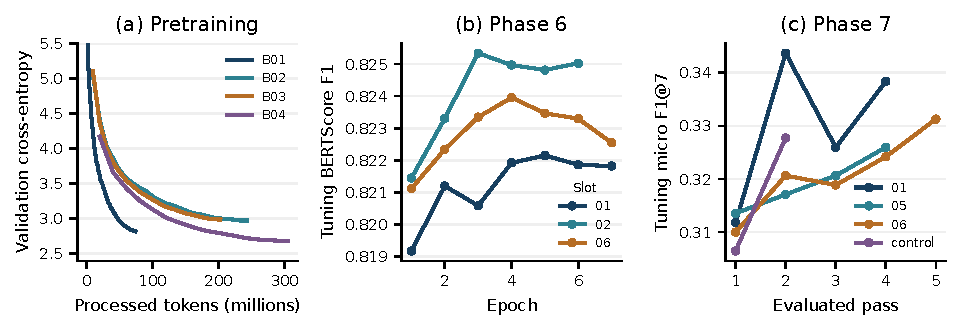
\includegraphics[width=\textwidth]{figures/learning_curves.pdf}
\caption{Saved learning curves. Pretraining protocols differ across bases, and the first plot displays loss below 5.5 for readability. Task curves show evaluated checkpoints; slot05 retrieval is incomplete in the archived run.}
\label{fig:curves}
\end{figure}

The lowest logged foundation losses are 2.82046, 2.97407, 2.98855 and 2.68014 for bases~01--04. Several task runs peak before their last epoch. The full retrieval model is best at pass~2, and the small KD advantage at pass~1 reverses at pass~2. Summarization gains are also small on the score scale. These curves explain why retaining the best checkpoint matters: a lower final training loss or a longer run does not guarantee a better submission.

\section{Error Analysis and Discussion}
\subsection{Phase-wise failure modes}
NER errors are concentrated in participant and witness spans. In the selected hybrid OOF predictions, APP has 76 true positives out of 407 gold entities and 342 predictions; RESP has 71 out of 381 gold and 376 predictions. Their F1 scores are 0.20294 and 0.18758, compared with 0.95907 for DATE. Only 111/407 APP and 122/381 RESP gold spans appear among the exact candidates. This puts a clear limit on threshold tuning: it cannot recover a span that is missing from the candidate set. The aggregate counts do not show the precise legal context behind each error.

Role prediction has a different problem: rare labels have very little independent support. All overruled-precedent examples come from one document. HighF1 raw decoding scores 0.42415 on document OOF and 0.53335 on dev when only supported labels are averaged; its fixed all-thirteen dev score is 0.45130. Pair corrections slightly improve supported dev F1 but lower OOF F1 to 0.42156, and CRF variants also trail raw OOF. This is a reason to be cautious about a small dev improvement.

The selected judgment model misses 502 positive outcomes and makes 355 false-positive predictions. Positive recall is 0.71412, compared with 0.79703 for the negative class. Chunk sampling could omit outcome-bearing text, but that explanation was not checked through manual examples. Duplicates and unfinished outer folds also limit the conclusion. In statutes, slot~01 predicts 4.92 labels per case against 3.68 gold, with subset accuracy 0.04143. Distillation reduces the predicted count to 4.80 and raises subset accuracy to 0.04515, with micro F1 0.47888. Both models still overpredict; calibration alone does not solve the long tail.

The summarization audit records 5,430 truncated fitting targets for base~03. Its audit outputs average 398.18 words, while references average 858.93, so a good embedding score can still hide missing content. Retrieval also has a structural limit: ten training queries have no relevant case, while others have more than seven. Even a perfect dev ranking can reach only 0.61812 under the seven-output rule. The neural views cover only part of very long candidates, although full-document BM25 still has access to their words.

\subsection{What the metrics do not measure}
The metrics capture only part of what a legal system needs to do. BERTScore measures contextual similarity and ROUGE measures lexical overlap~\cite{zhang2020bertscore,lin2004rouge}; neither checks whether the conclusion, citation or remedy is legally correct. Strict span F1 gives no partial credit for a nearly correct boundary. Macro F1 gives rare labels equal weight, but changes when absent labels are included or excluded. Retrieval micro F1@7 counts relevant pairs without distinguishing binding authority from a related case. Human legal review would still be needed.

\subsection{Limitations and what you would do next}
The official scores and ranks have been checked, but the local validation is incomplete in places. Phase~4 has no completed outer folds. The Phase~7 recovery is older than its standalone slot~05 package and has no final audit. All four foundation notebooks and the available alternatives are included, with archived runtimes kept where they differ from local files.

The next experiments should target these gaps: exact boundary generation for NER, whole-document generalization for roles and judgments, label-count control for statutes, and source/target budgets for summaries. Retrieval should complete its audit, then compare sparse, dense and fused rankings with the encoder held fixed.

\subsection{Surprising findings}
The results that did not improve were as useful as the gains. The NER reranker loses to calibrated raw V3 candidates. Role transitions look slightly better on the small dev set but worse on document OOF. The retrieval gold-only control overtakes KD at the second pass. Together, these results show why added complexity needs a matched comparison before it becomes part of the final system.

\section{Conclusion}
The project shows what can be built from four compact legal foundations under a fixed data and compute budget. Exact boundaries matter for NER, document context matters for roles, and lexical coverage remains useful for retrieval. Summarization has a completed independent audit; other tasks need stronger held-out checks. Across the experiments, more training and more elaborate decoding did not consistently produce better results. The most useful changes addressed a specific failure and were evaluated against a clearly defined baseline.

\par
\label{LastMainPage}
\typeout{MAIN_BODY_END_PAGE:\thepage}

\clearpage
\section*{LLM Usage Declaration}

\noindent\textbf{Q1.} Which Large Language Model(s), if any, did you use while completing the competition or writing this report?

\noindent\textbf{Answer:} I used GPT Sol 6 (OpenAI) to understand the project's concepts, discuss architecture and training plans, and interpret experimental results. It also assisted with implementation, debugging and report preparation, as recorded below. The downstream task models used the project's Phase~1 checkpoints rather than an external generative model as their backbone.

\medskip
\noindent\textbf{Q2.} For each row, mark Yes or No and state the purpose in one short phrase.

{\small
\setlength{\tabcolsep}{5pt}
\renewcommand{\arraystretch}{1.12}
\begin{longtable}{>{\raggedright\arraybackslash}p{3.9cm}>{\centering\arraybackslash}p{1.25cm}>{\raggedright\arraybackslash}p{9.7cm}}
\toprule
Part & Used LLM? & Purpose of using the LLM\\
\midrule
\endfirsthead
\toprule
Part & Used LLM? & Purpose of using the LLM\\
\midrule
\endhead
\bottomrule
\endfoot
Understanding concepts / papers & Yes & Explanations of byte-level BPE and character offsets; causal, encoder--decoder and prefix attention; RoPE, RMSNorm and grouped-query attention; LoRA, LoRMA, adapters, IA$^3$, prompts and distillation; BM25, chunk interaction, rank fusion, macro/micro F1 and BERTScore.\\
Ideation / brainstorming at a high level & Yes & Discussion of long-document chunking, task heads and sparse--dense retrieval.\\
Debugging small ancillary snippets & Yes & Explanation and correction of schema, CUDA-memory and recovery errors.\\
Plotting / visualization code & Yes & Figures and tables derived from saved experiment records.\\
Grammar / writing style of the report & Yes & Editing phrasing, notation and LaTeX presentation.\\
Report structure / section wording & Yes & Drafting and organizing material within the supplied template.\\
Designing the model architecture & Yes & Proposing and comparing backbone, task-head and adaptation choices.\\
Hyperparameter search / tuning & Yes & Suggested training settings, stopping rules and validation procedures.\\
Analysis of results / conclusions & Yes & Discussion and drafting of metric comparisons, failure analysis and limitations.\\
Writing the core training / inference code & Yes & Assistance with training/inference notebooks, evaluation and recovery logic.\\
Other (specify) & Yes & Repository documentation and final artifact packaging.\\
\end{longtable}
}

\noindent\textbf{Q3.} Did you refer to sources other than lecture slides and an LLM?

\noindent\textbf{Answer:} Yes. I used the official course specification, dataset, starter material and evaluation scripts, together with the architecture, adaptation, retrieval and metric papers cited in the bibliography. The implementation uses PyTorch, Hugging Face utilities, NumPy, SciPy and scikit-learn. Evaluation-model use is separate from task-model initialization.

\clearpage
\noindent\textbf{Q4.} Apart from LLM use, what was your contribution?

\noindent\textbf{Answer:} I set the project goals and requested efficient, resumable training across seven phases. I supplied the Phase~1 recoveries, previous notebooks and saved artifacts. I configured Kaggle GPUs, the HF\_TOKEN secret and persistence. I ran notebooks and supplied screenshots and logs when errors occurred. I downloaded and maintained recovery archives. I used explanations of tokenization, attention, adaptation and retrieval to support my understanding. I requested comparisons of the saved results and checks of updated artifacts. Retrieval memory exhaustion showed the need for representative batch probes and recovery. A missing fifth retrieval submission after the session budget expired showed the distinction between partial training and a completed package. The table above records the model assistance used alongside these activities.

\clearpage
\bibliographystyle{ieeetr}
\bibliography{references}
\end{document}
